	% XeLaTeX document
\documentclass[12pt,a4paper]{article}
% Редактируем: конфигурация, личные настройки: имя, название предмета и пр. для титульной страницы и метаданных документа здесь
\newcommand{\university}{Санкт-Петербургский политехнический университет Петра Великого}
\newcommand{\faculty}{Институт компьютерных наук и технологий}
\newcommand{\department}{Высшая школа интеллектуальный систем и суперкомпьютерных технологий}
\newcommand{\city}{Санкт-Петербург}
\newcommand{\docname}{Отчёт по лабораторной работе 12}
\newcommand{\subject}{Телекоммуникационные технологии}
\newcommand{\tutorname}{Н. В. Богач}
\newcommand{\studentname}{Д.А Ефимов}
\newcommand{\group}{3530901/00201}

% Не редактируем: используемые пакеты
% настройка кодировки, шрифтов и русского языка
\usepackage{fontspec}
\usepackage{polyglossia}

% рабочие ссылки в документе
\usepackage{hyperref}

% графика
\usepackage{graphicx}
\usepackage{tikz}

% поворот страницы
\usepackage{pdflscape}

% качественные листинги кода
\usepackage{minted}
\usepackage{lstfiracode}

\usepackage{listings}


\usepackage{xcolor}
%New colors defined below
\definecolor{codegreen}{rgb}{0,0.6,0}
\definecolor{codegray}{rgb}{0.5,0.5,0.5}
\definecolor{codepurple}{rgb}{0.58,0,0.82}
\definecolor{backcolour}{rgb}{0.95,0.95,0.92}

%Code listing style named "mystyle"
\lstdefinestyle{mystyle}{
  backgroundcolor=\color{backcolour}, commentstyle=\color{codegreen},
  keywordstyle=\color{magenta},
  numberstyle=\tiny\color{codegray},
  stringstyle=\color{codepurple},
  basicstyle=\ttfamily\footnotesize,
  breakatwhitespace=false,         
  breaklines=true,                 
  captionpos=b,                    
  keepspaces=false,                 
  numbers=left,                    
  numbersep=5pt,                  
  showspaces=false,                
  showstringspaces=false,
  showtabs=false,                  
  tabsize=2
}



% отключение копирования номеров строк из листинга, работает не во всех просмотрщиках (в Adobe Reader работает)
\usepackage{accsupp}
\newcommand\emptyaccsupp[1]{\BeginAccSupp{ActualText={}}#1\EndAccSupp{}}
\let\theHFancyVerbLine\theFancyVerbLine
\def\theFancyVerbLine{\rmfamily\tiny\emptyaccsupp{\arabic{FancyVerbLine}}}

% библиография
\bibliographystyle{templates/gost-numeric.bbx}
\usepackage{csquotes}
\usepackage[parentracker=true,backend=biber,hyperref=true,bibencoding=utf8,style=numeric-comp,language=auto,autolang=other,citestyle=gost-numeric,defernumbers=true,bibstyle=gost-numeric,sorting=ntvy]{biblatex}

% установка полей
\usepackage{geometry}

% нумерация картинок по секциям
\usepackage{chngcntr}

% дополнительные команды для таблиц
\usepackage{booktabs}

% для заголовков
\usepackage{caption}
\usepackage{titlesec}
\usepackage[dotinlabels]{titletoc}

% разное для математики
\usepackage{amsmath, amsfonts, amssymb, amsthm, mathtools}

% водяной знак на документе, см. main.tex
\usepackage[printwatermark]{xwatermark}

% Не редактируем: параметры используемых пакетов и не только
% настройки polyglossia
\setdefaultlanguage{russian}
\setotherlanguage{english}

% локализация
\addto\captionsrussian{
	\renewcommand{\figurename}{Рисунок}%
	\renewcommand{\partname}{Глава}
	\renewcommand{\contentsname}{\centerline{Содержание}}
	\renewcommand{\listingscaption}{Листинг}
}

% основной шрифт документа
\setmainfont{CMU Serif}
\newfontfamily\cyrillicfont{CMU Serif}[Script=Cyrillic]

% перечень использованных источников
\addbibresource{refs.bib}

% настройка полей
\geometry{top=2cm}
\geometry{bottom=2cm}
\geometry{left=2cm}
\geometry{right=2cm}
\geometry{bindingoffset=0cm}

% настройка ссылок и метаданных документа
\hypersetup{unicode=true,colorlinks=true,linkcolor=red,citecolor=green,filecolor=magenta,urlcolor=cyan,
	pdftitle={\docname},
	pdfauthor={\studentname},
	pdfsubject={\subject},
	pdfcreator={\studentname},
	pdfproducer={Overleaf},
	pdfkeywords={\subject}
}

% настройка подсветки кода и окружения для листингов
\usemintedstyle{colorful}
\newenvironment{code}{\captionsetup{type=listing}}{}

% шрифт для листингов с лигатурами
\setmonofont{FiraCode-Regular.otf}[
	SizeFeatures={Size=10},
	Path = templates/,
	Contextuals=Alternate
]

% оформления подписи рисунка
\captionsetup[figure]{labelsep = period}

% подпись таблицы
\DeclareCaptionFormat{hfillstart}{\hfill#1#2#3\par}
\captionsetup[table]{format=hfillstart,labelsep=newline,justification=centering,skip=-10pt,textfont=bf}

% путь к каталогу с рисунками
\graphicspath{{fig/}}

% Внесение titlepage в учёт счётчика страниц
\makeatletter
\renewenvironment{titlepage} {
	\thispagestyle{empty}
}
\makeatother

\counterwithin{figure}{section}
\counterwithin{table}{section}

\titlelabel{\thetitle.\quad}

% для удобного конспектирования математики
\mathtoolsset{showonlyrefs=true}
\theoremstyle{plain}
\newtheorem{theorem}{Теорема}[section]
\newtheorem{proposition}[theorem]{Утверждение}
\theoremstyle{definition}
\newtheorem{corollary}{Следствие}[theorem]
\newtheorem{problem}{Задача}[section]
\theoremstyle{remark}
\newtheorem*{nonum}{Решение}

% настоящее матожидание
\newcommand{\MExpect}{\mathsf{M}}

% объявили оператор!
\DeclareMathOperator{\sgn}{\mathop{sgn}}

% перенос знаков в формулах (по Львовскому)
\newcommand*{\hm}[1]{#1\nobreak\discretionary{} {\hbox{$\mathsurround=0pt #1$}}{}}



% водяной знак для обозначения статуса документа
% \newwatermark[allpages,color=red!5,angle=45,scale=3,xpos=0,ypos=0]{DRAFT}
\begin{document}
% Не редактируем: Титульная страница (формируется автоматически из заданной конфигурации)
\begin{titlepage}	% начало титульной страницы

	\begin{center}		% выравнивание по центру

		\large \university \\
		\large \faculty \\
		\large \department \\[6cm]
		% название института, затем отступ 6см

		\huge \subject \\[0.5cm] % название работы, затем отступ 0,5см
		\large \docname \num \\[5.1cm]
		% \large Тема работы\\[5cm]

	\end{center}


	\begin{flushright} % выравнивание по правому краю
		\begin{minipage}{0.25\textwidth} % врезка в половину ширины текста
			\begin{flushleft} % выровнять её содержимое по левому краю

				\large\textbf{Работу выполнил:}\\
				\large \studentname \\
				\large {Группа:} \group \\

				\large \textbf{Преподаватель:}\\
				\large \tutorname

			\end{flushleft}
		\end{minipage}
	\end{flushright}

	\vfill % заполнить всё доступное ниже пространство

	\begin{center}
		\large \city \\
		\large \the\year % вывести дату
	\end{center} % закончить выравнивание по центру

\end{titlepage} % конец титульной страницы

\vfill % заполнить всё доступное ниже пространство


% Не редактируем: Страница содержания (формируется автоматически из section, subsection и пр., указанных в content.tex)
% Содержание
\tableofcontents
\newpage



\lstset{style=mystyle}
% Редактируем: всё остальное: вступление, др. этапы, заключение, приложение
\section{FSK}
\subsection{Теоритическая основа}

\qquad Frequency Shift Key - вид модуляции, при которой скачкообразно изменяется частота несущего сигнала в зависимости от значений символов информационной последовательности. Частотная модуляция весьма помехоустойчива, так как помехи искажают в основном амплитуду, а не частоту сигнала.

\begin{figure}[H]
	\begin{center}
		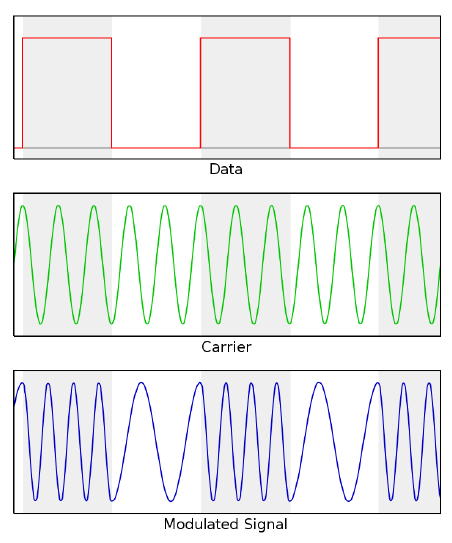
\includegraphics[scale=1]{fig/lab12/lab12_01.png}
		\caption{Пример FSK с двоичными данными}
	\end{center}
\end{figure}

\subsection{Схема в GNU Radio}    
    Для модулирования и тестирования данного процесса, необходимо построить следующую схему в графическом интерфейсе GNU Radio:
    
    \begin{landscape}
    	\begin{figure}[H]
        		\centering
        		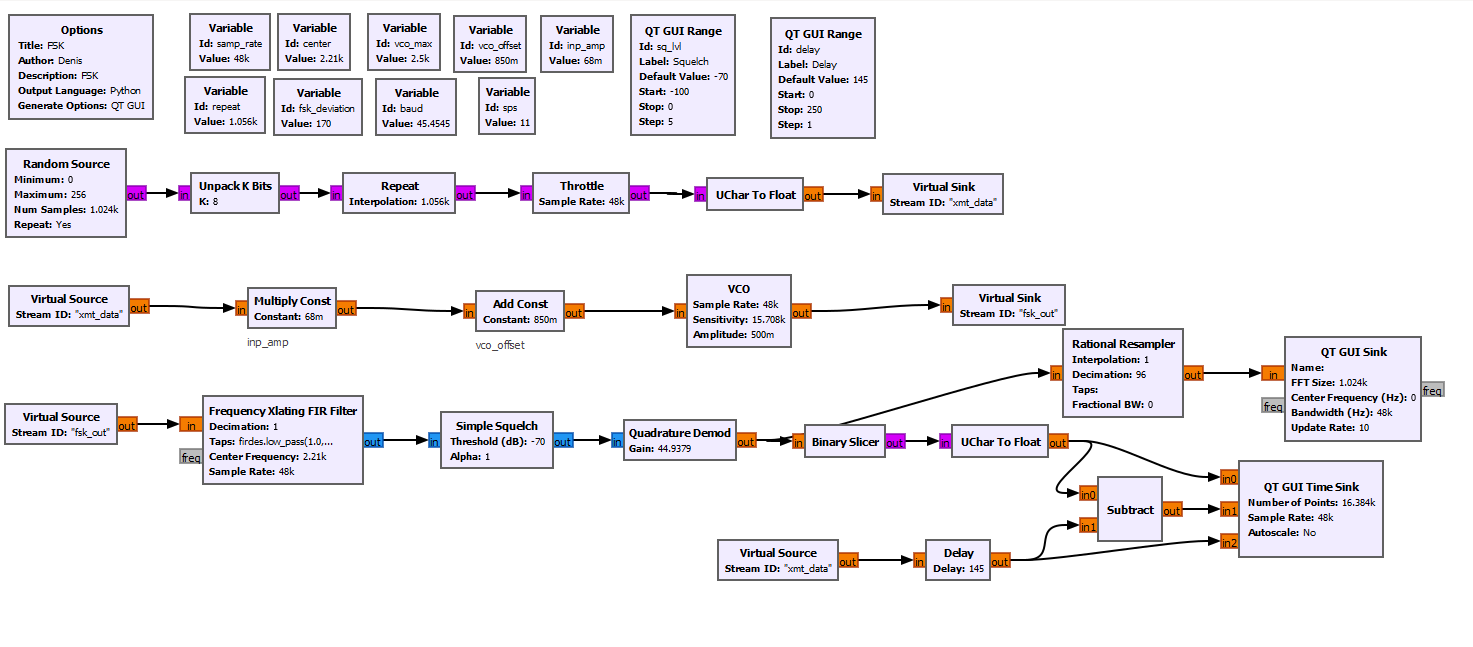
\includegraphics[width=25.5cm]{fig/lab12/lab12_02.png}
        		\caption{Схема FSK}
        		\label{pic:fsk_scheme} % название для ссылок внутри кода
    	\end{figure}
\end{landscape}

В данной схеме используются следующие блоки:
\begin{itemize}
	\item Frequency Xlating FIR Filter - Этот блок выполняет частотный перевод сигнала, а также понижает разрешение сигнала, запуская на нем децимирующий FIR-фильтр.
	\item Simple Squelch - Простой блок шумоподавления на основе средней мощности сигнала и порога в дБ.
	\item Quadrature Demod - Этот блок вычисляет произведение одновыборочного отложенного и сопряженного входного сигнала и нераскрытого сигнала, а затем вычисляет аргумент (также известный как угол, в радианах) результирующего комплексного числа.
	\item Binary Slicer - Нарезает числа с плавающей запятой, производя 1-битный вывод. Положительный ввод производит двоичную 1, а отрицательный ввод производит двоичный ноль. 
	\item QT GUI Sink - Выводы необходимой инфомрации в графическом интерфейсе.
    \item Options - Этот блок устанавливает некоторые общие параметры графа потоков. Такие как название проекта, авторство и другие. 
	\item Variable - Этот блок сопоставляет значение с уникальной переменной. Есть возможность использования переменной в другом блоке, благодаря идентификатору (id) блока переменных. 
	\item Multiply Const - Умножает входной поток на скалярную или векторную константу.
	\item Add Const - Прибавляет к входному потоку скалярную или векторную константу.
	\item QT GUI Range - Этот блок создает переменную с выбором виджетов. Переменной может быть присвоено значение по умолчанию, и ее значение может быть изменено во время выполнения в указанном диапазоне.
	\item Random Source - Генератор случайных чисел.
	\item Unpack K bits - Преобразует байт с k релевантных битов в k выходных байтов с 1 битом каждый.
	\item Repeat - Количество раз для повторения входных данных, выступающих в качестве коэффициента интерполяции.
	\item Throttle - Этот блок служит для того, чтобы дросселировать поток так, чтобы средняя скорость не превышала удельную скорость.
	\item Uchar To Float - Преобразует unsigned chars в поток float.
	\item Virtual Sink - Служит для сохранения потока в вектор.
	\item Virtual Source - Работает в паре с Virtual Sink блоком. Источник данных, который передаёт элементы на основе входного вектора. 
	\item VCO - Генератор с регулируемым напряжением. Создает синусоиду частоты на основе амплитуды входного сигнала.
\end{itemize}

В этом примере используется Baudot Radioteletype, следовательно битовое время = 22 миллисекунды. Получаем скорость передачи 45,4545.
Коэффицент повторения равен samp\_rate * 0,022.

В VCO генерируются сигналы 2295 Гц (отметка = 1) и 2125 Гц (отметка = 0). При выборе полной шкалы частоты 2500 Гц (vco\_max) для входа +1 чувствительность VCO = (2 * math.pi * 2500 / 1) = 15708. Можно использовать любую частоту выше 2295 Гц. 2500 Гц — хорошее круглое число. Глядя на вывод виртуального источника «xmt\_data», Mark = +1.0 и Space = 0.0. Частота отметки 2295 Гц создается вектором inp\_amp = (1,0 * 0,068) + vco\_offset = 0,918, что равно (2295/2500). Параметр отводов частотного Xlating FIR Filter равен 'firdes.low\_pass(1.0,samp\_rate,1000,400)'.

Теперь посмотрим, что у нас с данными:
\quad Источник генерирует случайные байты (от 0 до 255). Далее этот байт распоковывается в каждый бит становится байтом со значащим младшим разрядом. Для ограничения потока использует Throttle.
\quad Приёмник при помощи фильтра смещает принимаемый сигнал так, чтобы он был сосредоточен вокруг центральной частоты - между частотами Mark и Space. Шумоподавитель добавлен для реального приёма сигналов. Блок Quadrature Demod производит сигнал, который является положительным для входных частот выше нуля и отрицательным для частот ниже нуля. Когда данные доходят до Binary Slicer, то на выходе получает биты, это и есть наша полученная информация.


\subsection{Тестирование}
Запустим моделирование.

    \begin{figure}[H]
	\begin{center}
		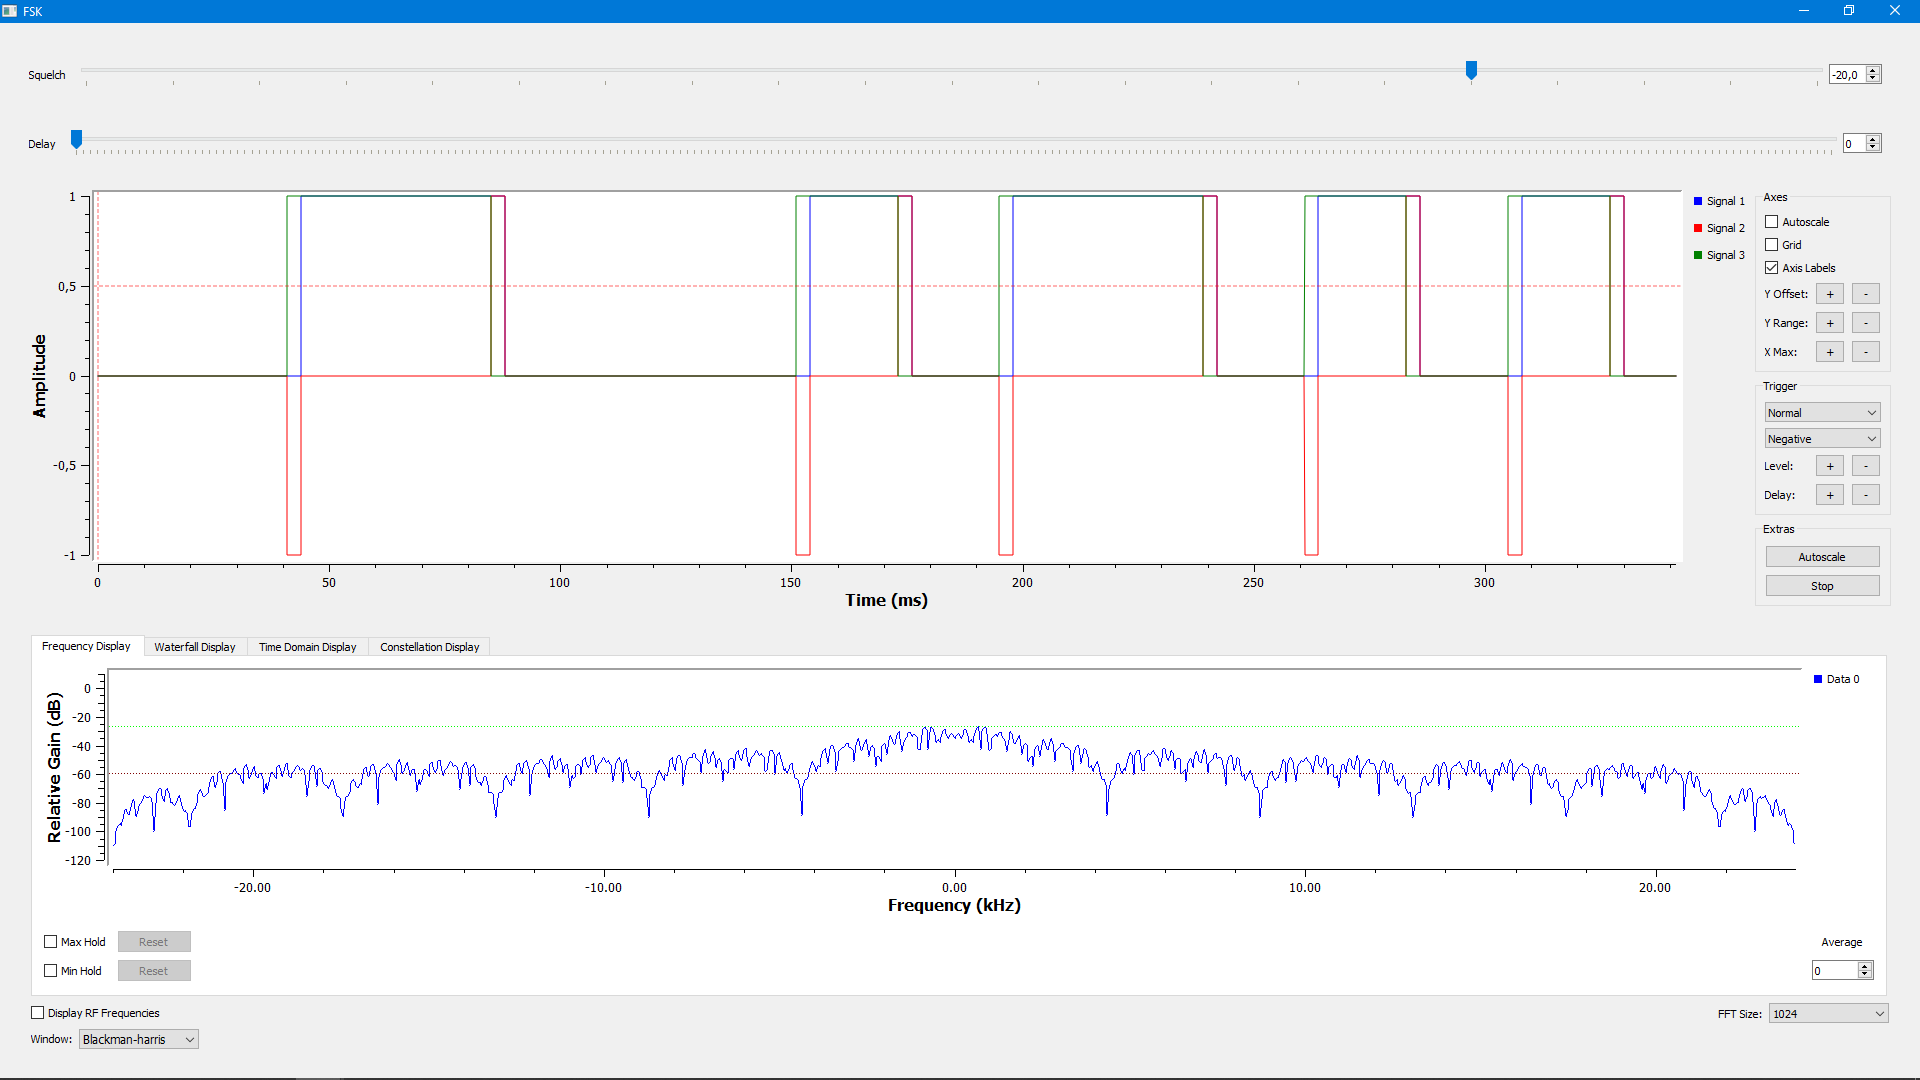
\includegraphics[scale=0.27]{fig/lab12/lab12_03.png}
		\caption{Тестирование без задержки с наложением шума}
		\label{pic:e1} % название для ссылок внутри кода
	\end{center}
\end{figure}

На графике можно видеть 3 сигнала разного цвета. Зеленный показывает данные которые были переданы передатчиком. Синий - это данные полученные приемником. А красный отвечает за разницу между зеленым и синим. Красный сигнал должен быть равен нулю, это сигнализирует о том, что данные передаются верно, однако на диаграмме сверху видно, что это не так и выходит так, что полученная информация различается от той, которую передавали. Принятый сигнал находится на некоторое количество бит позади, потому что цепочка передатчика и приемника имеет много блоков и фильтров, которые задерживают сигнал. Для того чтобы это исправить необходимо сделать задержку между приемом и передачей данных, что и обеспечивает блок Delay. Правильном задержкой является 145. 


    \begin{figure}[H]
	\begin{center}
		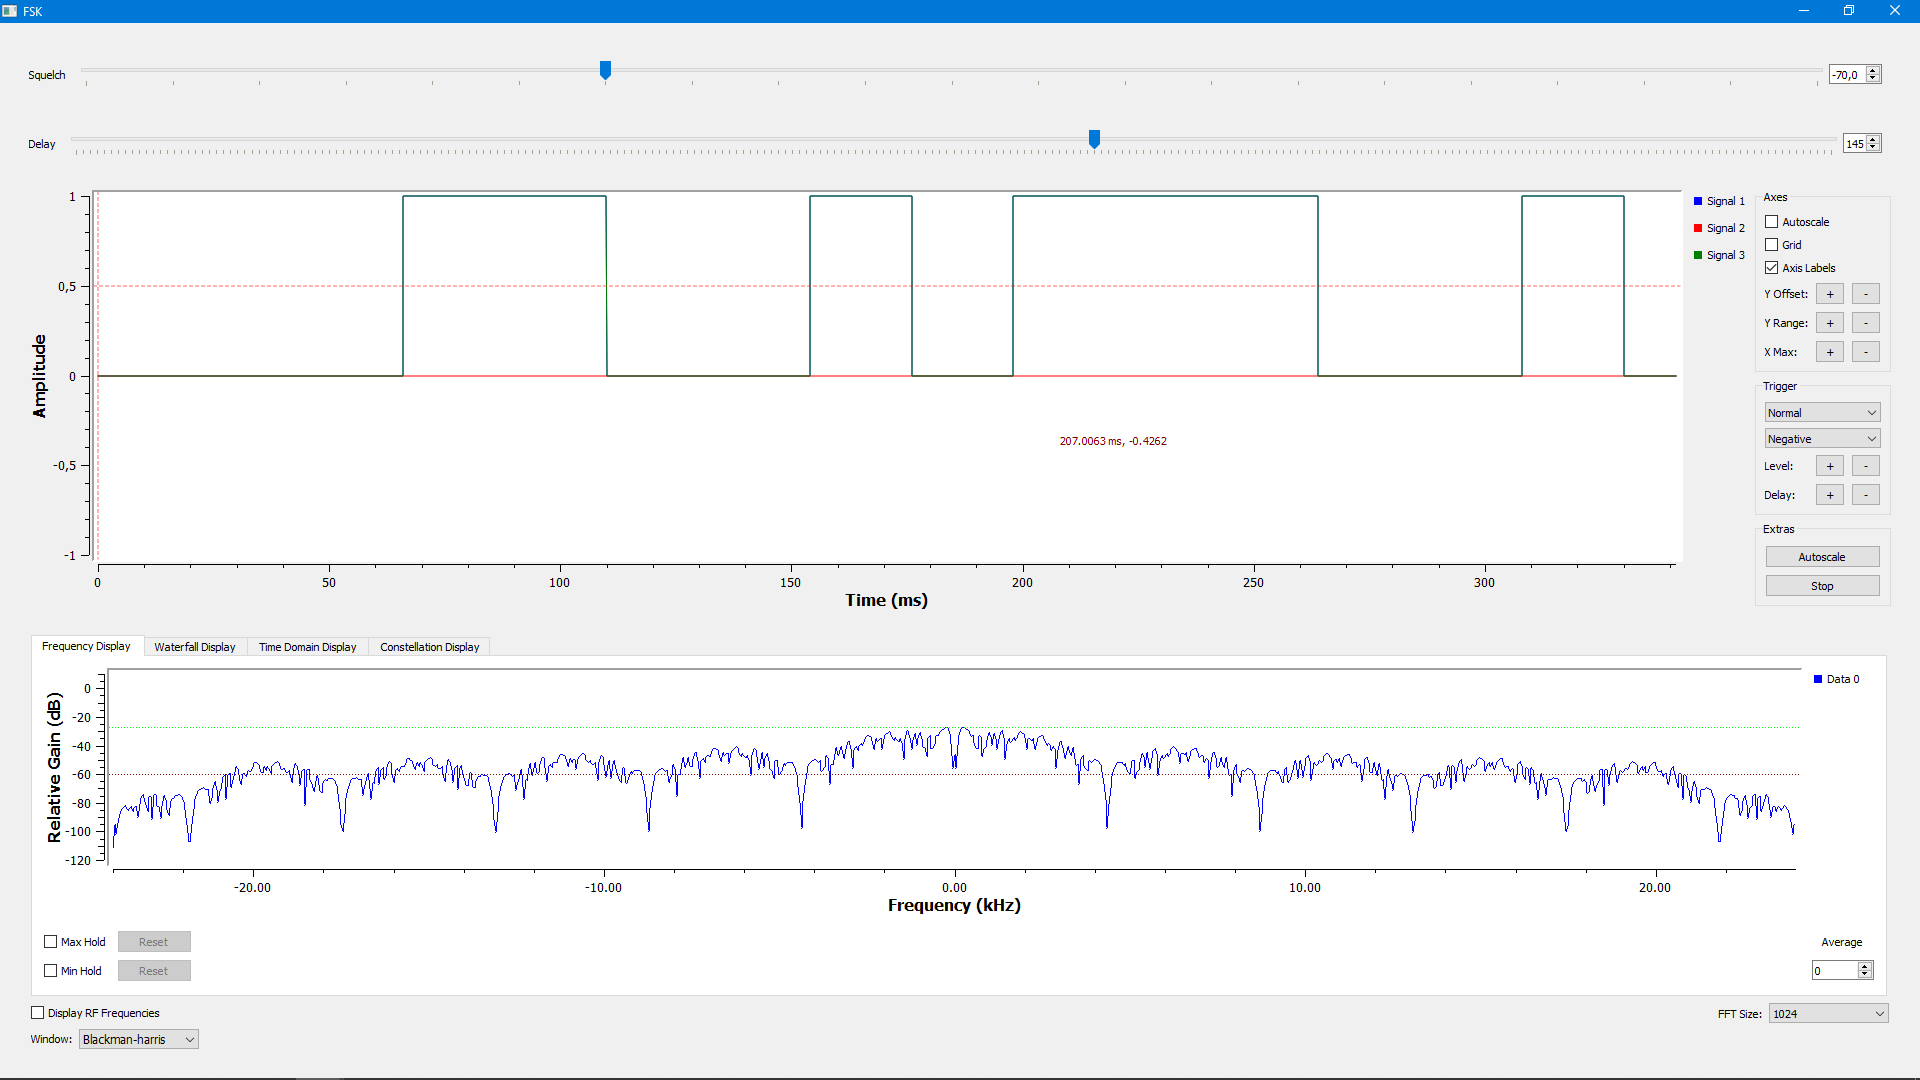
\includegraphics[scale=0.27]{fig/lab12/lab12_04.png}
		\caption{Тестирование с установленной задержкой}
		\label{pic:e1} % название для ссылок внутри кода
	\end{center}
\end{figure}

Теперь как можно заметить все хорошо и данные передаются и получаются корректно. 

\subsection{Вывод}
В данной лабораторной работе был рассмотрен один из способов модуляции. При помощи GNU Radio была создана и протестирована необходимая модель. 
\newpage

\addcontentsline{toc}{section}{Заключение}

% Не редактируем: Страница библиографии (формируется автоматически из книжек, указанных в refs.bib и пометок \cite{имя_источника} в тексте)
\newpage
\printbibliography[title=Перечень использованных источников]
\addcontentsline{toc}{section}{Перечень использованных источников}
\end{document}
